% !TeX program = xelatex
% !TeX encoding = UTF-8
\documentclass[UTF8]{standalone}
\usepackage{amsmath,fourier,ctex,tikz}
\begin{document}
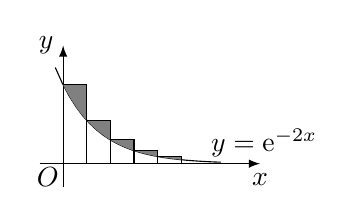
\begin{tikzpicture}
	\draw[-latex] (-0.3,0) node[left=-3pt,below=-2pt] {$O$} -- (2.5,0) node[below] {$x$};
	\draw[-latex] (0,-0.3) -- (0,1.5) node[left] {$y$};
	\draw[domain=-0.1:2] plot (\x,{exp{-2*\x}}) node[above=7pt,right=-7pt] {$y = \mathrm{e}^{-2x}$};
	\fill [fill = gray] [domain = 0:0.3,smooth] plot (\x, {exp{-2*\x}}) -- (0.3,1)  -- cycle;
	\fill [fill = gray] [domain = 0.3:0.6,smooth] plot (\x, {exp{-2*\x}}) -- (0.6,{exp{-2*0.3}})  -- cycle;
	\fill [fill = gray] [domain = 0.6:0.9,smooth] plot (\x, {exp{-2*\x}}) -- (0.9,{exp{-2*0.6}})  -- cycle;
	\fill [fill = gray] [domain = 0.9:1.2,smooth] plot (\x, {exp{-2*\x}}) -- (1.2,{exp{-2*0.9}})  -- cycle;
	\fill [fill = gray] [domain = 1.2:1.5,smooth] plot (\x, {exp{-2*\x}}) -- (1.5,{exp{-2*1.2}})  -- cycle;
	\draw (0,1) -- ++ (0.3,0) -- ++ (0,-1);
	\draw (0.3,{exp{-2*0.3}}) -- ++ (0.3,0) -- ++ (0,-{exp{-2*0.3}});
	\draw (0.6,{exp{-2*0.6}}) -- ++ (0.3,0) -- ++ (0,-{exp{-2*0.6}});
	\draw (0.9,{exp{-2*0.9}}) -- ++ (0.3,0) -- ++ (0,-{exp{-2*0.9}});
	\draw (1.2,{exp{-2*1.2}}) -- ++ (0.3,0) -- ++ (0,-{exp{-2*1.2}});
\end{tikzpicture}
\end{document}